% Created 2024-09-02 Mon 23:51
% Intended LaTeX compiler: pdflatex
\documentclass[letterpaper, 12pt]{article}
\usepackage[utf8]{inputenc}
\usepackage[T1]{fontenc}
\usepackage{graphicx}
\usepackage{longtable}
\usepackage{wrapfig}
\usepackage{rotating}
\usepackage[normalem]{ulem}
\usepackage{amsmath}
\usepackage{amssymb}
\usepackage{capt-of}
\usepackage{hyperref}
\usepackage{minted}
\usepackage{xcolor}
\usepackage{hyperref}
\usepackage{tocloft}
\usepackage{minted}
\usemintedstyle{manni}
\usepackage{pdfpages}
\usepackage{fancyhdr}
\usepackage{graphicx}
\usepackage[top=1.4in, left=0.5in, right=0.5in, bottom=0.8in]{geometry}
\usepackage[T1]{fontenc}
\usepackage{helvet}
\pagestyle{fancy}
\renewcommand{\headrulewidth}{0pt}
\renewcommand{\footrulewidth}{0pt}
\setlength{\parindent}{0em}
\setlength{\parskip}{1em}
\usepackage{hyperref}
\usepackage {color}
\usepackage {tabularray}
\usepackage{xcolor}
\hypersetup{
colorlinks=true,
linkcolor=blue,
filecolor=magenta,
urlcolor=cyan,
citecolor=green,
pdfborder={0 0 0}
}
\usepackage[most]{tcolorbox}
\author{Hilduara Abreu}
\date{2024-09-05}
\title{School Year 2024-25 | PS 192 Visitor and Safety Guidelines and Procedures}
\hypersetup{
 pdfauthor={Hilduara Abreu},
 pdftitle={School Year 2024-25 | PS 192 Visitor and Safety Guidelines and Procedures},
 pdfkeywords={},
 pdfsubject={},
 pdfcreator={Emacs 29.4 (Org mode 9.6.15)}, 
 pdflang={English}}
\begin{document}

\fancyfoot[C]{\setlength{\unitlength}{1in}\begin{picture}(5,0)\put(-1.8,-0.5){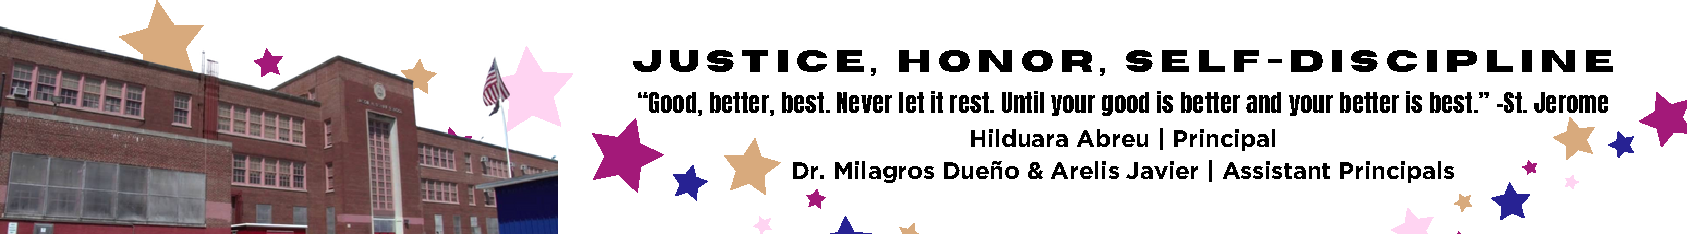
\includegraphics[width=8.8in,height=1.3in]{logo-1}}\end{picture}}
\fancyhead[C]{\setlength{\unitlength}{1in}\begin{picture}(5,0)\put(-1.9,-0.5){
\includegraphics[width=8.9in,height=1.3in]{logo-2}}\end{picture}}
\fancyhead[R]{\thepage}
\pagenumbering{gobble}

\begin{document}
\newpage
\vspace*{-0.5cm}
\textbf{School Year 2024-25 | PS 192 Visitor and Safety Guidelines and Procedures}

\textbf{Dear Parents or Guardians},

We are pleased to present the guidelines and procedures for our esteemed institution, Jacob H. Schiff/P.S. 192. These guidelines and procedures have been meticulously designed to prioritize the safety and security of all individuals—our valued students, dedicated staff, and respected visitors—while fostering an environment that is welcoming and inclusive. We sincerely appreciate your cooperation in adhering to these essential protocols.

\textbf{Visitor Arrival}
\begin{itemize}
\item Upon Arrival: All visitors, including parents, guardians, volunteers, contractors, and esteemed guests, are kindly requested to enter the school premises through the main entrance and proceed to the safety agent desk for registration.
\item Warm Welcome: Our School Safety Agent or designated school staff will warmly welcome all visitors, inquire about the purpose of your visit, and request a valid photo ID.
\item Identification: To ensure security, visitors must present a valid form of identification, such as a driver’s license, government-issued ID, foreign or US passport, or consulate identification card. Subsequently, visitors will be given an identification sticker, which must be prominently displayed throughout their visit. The School Safety Agent will assist in issuing the identification sticker.
\item Assistance Notification: Once the School Safety Agent or designated school staff completes the registration process, they will notify Ms. Rijo, our parent coordinator, by calling X1190. This will facilitate further assistance for the visitor, whether waiting in the lobby or the auditorium.
\end{itemize}

\textbf{Scheduled Visits}

We encourage non-emergency visits to be scheduled whenever possible to ensure that staff members are available to meet with visitors and minimize disruption to instructional time. Visitors and staff can schedule appointments through various channels, including Classdojo, staff direct email, our school website, or by contacting the parent coordinator.
\begin{itemize}
\item Visitor Arrival: Upon arriving for a scheduled appointment, visitors are kindly requested to follow the same entrance and registration process outlined above.
\end{itemize}

\textbf{Escort and Supervision}

For added security, a designated staff member will escort visitors to and from their intended destination \newpage \vspace*{-0.5cm} within the school premises, including classrooms, offices, the library, the gym, and other shared spaces. - Supervised Contact: Visitors should interact with students only if expressly authorized by school administration or as part of a pre-approved program or event.

\textbf{Confidentiality and Privacy}

To uphold our students and staff members’ privacy and confidentiality, visitors are kindly requested not to take photographs or record videos while on school premises.
\begin{itemize}
\item Respect for Privacy: Any personal information or observations made during the visit should not be shared without appropriate consent or authorization from the NYC DOE.
\end{itemize}

\textbf{Safety Drills}

Throughout the academic year, we conduct safety drills to ensure that students and staff are well-prepared to respond effectively in emergencies. These drills are essential for the safety and security of our school community and include:
\begin{itemize}
\item 12 Fire Drills: Conducted bi-weekly from September to December 31, 2024, and monthly thereafter.
\item Lockdown Drills: Conducted every other month.
\item 2 Bus Emergency Drills: Conducted at the beginning of the school year (September 2024) and the start of the second semester (February 2025).
\end{itemize}

\textbf{Over-the-Phone Interpretation Services}

When a visitor speaks a language other than English, our School Safety Agent (SSA) or designated school staff member will try to identify the visitor’s language using the multi-language poster displayed at the safety desk. Once the language is ascertained, the visitor will be directed to Ms. Rijo, our parent coordinator, for further assistance. In cases where we do not have a staff member proficient in the visitor’s language on-site, the staff member will engage the DOE’s Over-the-Phone Interpretation Unit to arrange an on-demand interpreter.

\textbf{Departure}

All visitors must be accompanied by a staff member at ALL times until the visitor leaves the premises. This means that at the conclusion of the visit, the staff member must escort the visitor(s) to the main entrance to ensure departure.
\newpage \vspace*{-0.5cm}
Visitors are kindly requested to sign out with the School Safety Agent or designated school staff upon leaving the building. The identification sticker must be returned. All visitors must exit the building through the main entrance.

\textbf{Closing}

By faithfully following these visitor guidelines and procedures, we collectively contribute to our esteemed school community’s safety, security, and well-being. If you have any questions or require further clarification, please do not hesitate to contact us or contact Ms. Rijo at 646-745-0150 or 212-775-9560 X1190.

Your unwavering commitment and support are pivotal in maintaining a positive and secure learning environment. Additional assistance is also available through our website or WhatsApp.

Once again, we extend our heartfelt gratitude for your cooperation and dedication to our shared mission.

With Justice, Honor, and Self-Discipline,


\includegraphics[width=0.2\textwidth]{hil_signature}

\textbf{Hilduara Abreu, Principal}

\textbf{The school of Joyful Learning!}

\href{www.ps192.org}{www.ps192.org}
\end{document}
